\documentclass{beamer}

\usepackage[utf8]{inputenc}
% \usepackage[french]{babel}
\usepackage{etex}
% \usepackage[hidelinks]{TUL/tulhypref}
% \usepackage[sc]{mathpazo}
\linespread{1.0}
% Si on veut le style de bibliographie named :
%\usepackage{named}

% Pour les figures :
\usepackage{graphicx}

% Si on veut des mini-tables des matières (utiliser minitoc-hyper 
% en conjonction avec tulhypref) :
\usepackage[french]{minitoc}

% \usepackage{titlesec}
\usepackage{url}
\usepackage{listings}
\usepackage{pstricks}
\usepackage{subfigure}
\usepackage{amsmath}
\usepackage{amsthm}
\usepackage{amssymb}
\usepackage{tabularx}
\usepackage{textcomp}
\usepackage{multirow}
\usepackage[algoruled,french,onelanguage]{algorithm2e}
\usepackage[section]{placeins}
\usepackage{xcolor}
\usepackage{colortbl}
\usepackage{longtable}
\usepackage{booktabs}
% \setlength{\aboverulesep}{0pt}
% \setlength{\belowrulesep}{0pt}

\usepackage{epstopdf}
\usepackage{graphicx} % pour insérer des images
\usepackage{stmaryrd}
\usepackage{amsfonts}
% \usepackage{tikz}
% \usepackage{tikz-qtree}
% les figure imbriquées
\usepackage{epsfig}
\usepackage{enumerate}
\usepackage{pifont}
\usepackage{lscape}

\usepackage{pgf}
\usepackage{tikz, calc}
% \usepackage{tikz-cd}
\usetikzlibrary{positioning}
\usetikzlibrary{fit}
\usetikzlibrary{shapes.multipart,calc}
\usetikzlibrary{arrows}

% \usepackage[math]{iwona} 
% \usepackage{iwona} 
% \SetMathAlphabet{\mathtt}{iwona}{OT1}{\ttdefault}{m}{n}

\usepackage[backend=biber, language=french, maxnames=10, citestyle=alphabetic,bibstyle=alphabetic,backref,abbreviate=false,dateabbrev=false,isbn=false,url=false,doi=true]{biblatex}
% \usepackage[backend=biber, language=french, maxnames=5,backref,abbreviate=false,dateabbrev=false,isbn=false,url=false,doi=true]{biblatex}
\addbibresource{these.bib}
% \usepackage[font=small,skip=0pt]{caption}
\usepackage[skip=0pt]{caption}
\usepackage{etoolbox}
\usepackage{needspace}
% \usepackage[zerostyle=a]{newtxtt}

\newcounter{chapter}
% Todo
% \newcommand{\done}[1]{}
% \newcommand{\idone}[1]{}
\newcommand{\itodo}[1]{\todo[inline]{#1}}

\newcommand{\done}[1]{\todo[color=green!80!blue!80]{#1}}
\newcommand{\idone}[1]{\todo[inline,color=green!80!blue!80]{#1}}

\newcommand{\jym}[1]{\todo[color=red!80!blue!50]{#1}}
\newcommand{\ijym}[1]{\todo[inline,color=red!80!blue!50]{#1}}

\newcommand{\more}[1]{\todo[color=purple!60!blue!30]{#1}}
\newcommand{\imore}[1]{\todo[inline,color=purple!60!blue!30]{#1}}

% Samples
\newcommand{\telock}{tElock}

% Color cells
\newcommand{\cnoir}{\cellcolor[gray]{0.0}}
\newcommand{\cgris}{\cellcolor[gray]{0.8}}

% Traductions
\newcommand{\Layer}{Couche}
\newcommand{\Layers}{Couches}
\newcommand{\layer}{couche}
\newcommand{\layers}{couches}
% \newcommand{\Layer}{Strate}
% \newcommand{\Layers}{Strates}
% \newcommand{\layer}{strate}
% \newcommand{\layers}{strates}

% sm
\newcommand{\sm}{auto-modifiant}
\newcommand{\nsm}{non auto-modifiant}

% Structure
\newtheorem{pb}{Problème}
\newtheorem{theo}{Théorème}
\newtheorem{defi}{Définition}[chapter]
\newtheorem{prop}{Proposition}
\newtheorem{propri}{Propriété}
\newtheorem{pr}{Preuve}
\newtheorem{cor}{Corollaire}
\newtheorem{rem}{Remarque}
% \theoremstyle{remark}\newtheorem*{preuve}{Preuve}


% % Abbreviations :
\newcommand{\helloworld}{\texttt{Hello World}}
\newcommand{\nasm}{NASM}
\newcommand{\xq}{x86}
\newcommand{\xs}{x86$\_$64}
\newcommand{\pdata}{\texttt{.data}}
\newcommand{\ptext}{\texttt{.text}}

% Adresses mémoire :
\newcommand{\adr}[1]{$#1$}

% Registres
\newcommand{\eax}{\texttt{eax}}
\newcommand{\ebx}{\texttt{ebx}}
\newcommand{\ecx}{\texttt{ecx}}
\newcommand{\edx}{\texttt{edx}}
\newcommand{\edi}{\texttt{edi}}
\newcommand{\eip}{\texttt{eip}}
\newcommand{\esp}{\texttt{esp}}

% Instructions
\newcommand{\mov}{\texttt{mov}}
\newcommand{\cmp}{\texttt{cmp}}
\newcommand{\add}{\texttt{add}}
\newcommand{\jmp}{\texttt{jmp}}
\newcommand{\ret}{\texttt{ret}}
\newcommand{\call}{\texttt{call}}
\newcommand{\push}{\texttt{push}}
\newcommand{\jne}{\texttt{jne}}
\newcommand{\je}{\texttt{je}}
\newcommand{\sub}{\texttt{sub}}
\newcommand{\dec}{\texttt{dec}}
\newcommand{\nop}{\texttt{nop}}
\newcommand{\halt}{\texttt{halt}}
\newcommand{\pc}{\texttt{pc}}

% Sémantique statique
\newcommand{\BN}{\mathbb N}
\newcommand{\BE}{\mathbb E}
\newcommand{\BV}{\mathbb V}
\newcommand{\BX}{\mathbb X}
\newcommand{\BA}{\mathbb A}
\newcommand{\BP}{\mathbb P}
\newcommand{\BT}{\mathbb T}
\newcommand{\BL}{\mathbb L}
\newcommand{\BB}{\mathbb B}
\newcommand{\BNB}{\mathbb N\cup\{\bot\}}
\newcommand{\PN}{\mathcal{P}(\BN)}
\newcommand{\PMN}{\mathcal{P}_M(\BN)}
\newcommand{\Trs}{\mathbb N\cup\{\bot,\top\}}
\newcommand{\TTrs}{\mathcal P(\mathbb V\rightarrow\mathbb N\cup\{\bot,\top\})}
\newcommand{\Tr}{\PN\cup{\top,\bot}}
\newcommand{\TrM}{\PMN\cup\{\top,\bot\}}
\newcommand{\si}{\sigma_{init}}
\newcommand{\specialcell}[2][c]{%
  \begin{tabular}[#1]{@{}l@{}}#2\end{tabular}}
  
% Sémantique dynamique
\newcommand{\CA}{\mathcal A}
\newcommand{\CI}{\mathcal I}
\newcommand{\CC}{\mathcal C}
\newcommand{\CR}{\mathcal R}
\newcommand{\CW}{\mathcal W}
\newcommand{\da}[1]{$\CA[#1]$}
\newcommand{\di}[1]{$\CI[#1]$}
\newcommand{\dc}[1]{$\CC[#1]$}
\newcommand{\dr}[1]{$\CR[#1]$}
\newcommand{\dw}[1]{$\CW[#1]$}
\newcommand{\dww}[2]{$\CW^{#1}[#2]$}

% tikz
\tikzset{
  state/.style={
    rectangle,
    rounded corners=1pt,
    draw=black, very thick,
    minimum height=2em,
    text centered,
  },
}

% itemize
% \renewcommand{\labelitemii}{$\cdot$}
% \renewcommand{\labelitemi}{$\bullet$}
% \renewcommand{\labelitemii}{$\cdot$}
% \renewcommand{\labelitemiii}{$\diamond$}
% \renewcommand{\labelitemiv}{$\ast$}
% \usepackage{default}

% \usepackage{graphicx} % pour insérer des images
%\usepackage{graphics} % pour insérer des images vectorielles (ps, eps)
% \usepackage{epstopdf}

% les figure imbriquées
% \usepackage{epsfig}
% \usepackage{subfigure}



% \newtheorem{de}{Définition}
\setbeamertemplate{navigation symbols}{}
% \setbeamercolor{structure}{fg=black!90}
% \setbeamercolor*{palette primary}{use=structure,fg=white,bg=gray!60}
% \setbeamercolor*{palette quaternary}{fg=white,bg=gray!30!black}
% \newtheorem{prop}{Property}

% \usetheme{Warsaw}
 \usetheme{Frankfurt}
 \setbeamertemplate{title page}[default][rounded=false]
 \setbeamertemplate{frametitle}[default][colsep=-3bp,rounded=false,shadow=false]
% \usecolortheme{wolverine}
%   \usetheme{Berlin}
% \setbeamertemplate{footnote}{%
%   \hangpara{2em}{1}%
%   \makebox[2em][l]{\insertfootnotemark}\footnotesize\insertfootnotetext\par%
% }


\mode<presentation>{
\setbeamertemplate{footline}[frame number] %les numéros de page
\setbeamertemplate{bibliography item}[text]
} 
\title[Désassemblage et détection de logiciels malveillants auto-modifiants]{Désassemblage et détection de logiciels malveillants auto-modifiants}
\author{Aurélien \textsc{Thierry}}% (aurelien@athierry.fr)\\ Équipe CARTE\\ Sous la direction de Jean-Yves Marion}
%\institute{INRIA, Loria}
\date{11 mars 2015}
% \titlegraphic{\includegraphics[width=0.1\textwidth]{../images/loria.jpg}}
% \titlegraphic{\includegraphics[width=0.1\textwidth]{../images/logo_inria.jpg}}


\begin{document}
\makeatletter
  \@ifundefined{inserttotalframenumbernew}{
    \gdef\inserttotalframenumbernew{1}
  }{}
  \gdef\inserttotalframenumber{\inserttotalframenumbernew}
\makeatother


\begin{frame}[plain]
\titlepage
\begin{figure}[ht]
\begin{center}
  \subfigure{
\label{fig:CFGConstr}
\epsfig{figure=TUL/Inria.png,height=1.2cm}}\quad
  \subfigure{
\label{fig:CFGNorm}
\epsfig{figure=TUL/tulloria.pdf,height=1.3cm}}\
\subfigure{
\label{fig:CFGConstr}
\epsfig{figure=TUL/tulul.pdf,height=1.0cm}}\quad
\end{center}
\label{fig:CFGConstrNorm}
% \caption{Virut.a without (99 nodes) and with (41 nodes) reduction}
\end{figure}
\end{frame}

\section{Introduction}
% Les deux problèmes que l'on aborde dans cette thèse
% Todo : séparer le pb du domaine de ce qu'on a fait ?
\begin{frame}{Introduction}
Analyse de programmes binaires obscurcis
\begin{itemize}
 \item Désassemblage : séparation du code et des données
 \item Reconstruction du graphe de flot de contrôle (GFC)
\end{itemize}

Détection de programmes malveillants et analyse de similarités logicielles
\begin{itemize}
 \item Comparaison des graphes de flot de contrôle
 \item Formalisation et optimisation
\end{itemize}

\end{frame}

% \begin{frame}{Analyse de binaires}
% \begin{itemize}
%  \item 
% \end{itemize}
% \end{frame}

% \begin{frame}{Détection de similarités}
% \begin{itemize}
%  \item 
% \end{itemize}
% \end{frame}
% 
% \begin{frame}{Organisation et contributions}
% 
% \end{frame}

\section{Obscurcissement et désassemblage}
\subsection{Difficultés}

\lstdefinestyle{verbo}{
    basicstyle=\scriptsize\ttfamily,
    breaklines=true,
    breakatwhitespace=true,
    tabsize=1,
    resetmargins=true,
    xleftmargin=0pt,
    frame=none,
    showspaces=false,
    showstringspaces=false
}

\begin{frame}[fragile]{Compilation et binairea}
\begin{block}{Code C}
\begin{lstlisting}[language={C}, style=verbo]
printf("Hello, world.");
\end{lstlisting}
\end{block}

\begin{center}
\scalebox{1}{
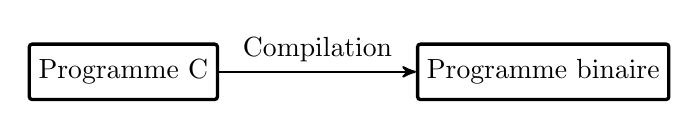
\begin{tikzpicture}[->,scale=1,>=stealth',thick]
\newcommand\espace{0.3cm}
\node[state] (PC) {Programme C};
\node[state, right=2.5cm of PC] (BIN) {Programme binaire};

% \draw [-] (PC) -- (BIN) {Compilation};
\draw (PC) -- node[above]{Compilation} (BIN);
\end{tikzpicture}}
\end{center}
\end{frame}

\begin{frame}{}

\begin{frame}{Graphe de flot de contrôle}

\end{frame}

\begin{frame}{Chevauchement de code}

\end{frame}

\begin{frame}{Auto-modification}

\end{frame}

\subsection{Sémantiques}
\begin{frame}{Traitement de l'auto-modification}

\end{frame}

\begin{frame}{Traitement du chevauchement de code (original)}

\end{frame}

\subsection{Notre approche}
\begin{frame}{Graphe de flot de contrôle parfait}

\end{frame}

\begin{frame}{Graphe de flot de contrôle paramêtré}

\end{frame}

\begin{frame}{Codisasm}

\end{frame}

\section{Algorithmes de comparaison}
\subsection{Analyse morphologique}
\begin{frame}{Détection de similarités logicielles}

\end{frame}

\subsection{Formalisation et simplification}
\begin{frame}{Isomorphisme appliqué aux graphes de flot}

\end{frame}

\subsection{Algorithmes et implémentation}
\begin{frame}{Algorithme par parcours}

\end{frame}

\begin{frame}{SIDT}

\end{frame}

\begin{frame}{Comparaison des performances}

\end{frame}

\begin{frame}{Implémentations}

\end{frame}

\section{Exemples d'application}

\begin{frame}{OpenSSL / Waledac}

\end{frame}

\begin{frame}{Duqu / Stuxnet}

\end{frame}

\section{Conclusion}

\begin{frame}{Conclusion}
\begin{itemize}
\item Analyse et désassemblage de programmes binaires obscurcis
\item Détection de similarités par comparaison des graphes de flot de contrôle
\item Application sur quelques cas de programmes malveillants
\end{itemize}
% Still to be done :
\pause
\begin{itemize}
\item Merci
\item Des questions ? (aurelien@athierry.fr)
% \item Loop detection and comparison for dynamic analysis
% \item Better reductions to detect through obfuscation
% \item Smoother UI for the IDA plugin
\end{itemize}
\end{frame}



\makeatletter
  \immediate\write\@mainaux{\string\gdef\string\inserttotalframenumbernew{\insertframenumber}}
\makeatother
\appendix


% \begin{frame}[allowframebreaks]
% \section*{}
% {
% \frametitle{Références}
% \bibliography{../rapportbib}
% \bibliographystyle{alpha}
% }
% \end{frame}

% % suppléments :
% \begin{frame}{More}
% \end{frame}




\end{document}
